% Chapter Template

\chapter{Background} % Main chapter title

\label{Chapter3} % Change X to a consecutive number; for referencing this chapter elsewhere, use \ref{ChapterX}

\lhead{Chapter 3. \emph{Background}} % Change X to a consecutive number; this is for the header on each page - perhaps a shortened title

%----------------------------------------------------------------------------------------
%	SECTION 1
%----------------------------------------------------------------------------------------

\section{Introduction}\label{Lit:Intro}
In this section, I will layout the key ideas and technologies which have inspired and enabled the research presented later in this thesis.

Due to the broad scope of the research carried out, the background section is loosely presented so as to compare and contrast the state-of-the-art artificial neural network technologies with their biological analogues (where possible). As such, I survey machine learning, robotics, psychology and biology literature. This is done to illuminate the thought process behind the choices I made in designing the experiments and \acp{ANN} in this thesis.

%This chapter aims to demonstrate how \acp{ANN} have very good performance in specific areas, whilst lagging far behind in many others. By bringing these divergent fields together, perhaps it is possible to find ways to improve \acp{ANN} whilst also further developing our understanding of what makes humans tick. 

As \acp{ANN} are my method of choice for implementing \ac{MRL} it is important to understand where they excel, as well as their limitations.

\section{What are Artifical Neural Networks Good at?}

Artificial Neural Networks have been around for a long time but perhaps the best example of early neural networks is the \acl{MLP}(\ac{MLP} \cite{rosenblatt1958perceptron}. Modern \acp{ANN} can trace their lineage back to the \ac{MLP}; however the technology has advanced a lot since 1958. \acp{ANN} represent the state-of-the-art on many Artificial Intelligence benchmarks.

\acp{ANN} are currently enjoying a new renaissance due to wide spread availablity of \acp{GPU}, big data, and software libraries like Tensorflow and CUDA.

In 2012, Krizhevsky et al. \cite{krizhevsky2012imagenet} kickstarted this new wave of interest in \acp{ANN} by getting the top performance on the ILSVRC-2012 ImageNet challenge. The unprecendented performance was achieved by utilising a very large amount of training data (1.2 million images), which was made possible by utilising the parallel computing power of \acp{GPU}. In creating AlexNet, Krizhevsky et al. demonstrated the potential of \acp{ANN} to solve real world problems, something which had been promised since \ac{ANN} research began.

The field of \ac{DL} has advanced greatly in recent years, with \acp{ANN} being used to solve many different types of problems. \ac{DL} is being used for many differnt tasks which can be broken down into several categories: Classification, \ac{NLP}, Data Generation, Reinforcement Learning \cite{vinyals2019alphastar} and Prediction Tasks.


Of these categories of problems, \ac{MRL}(as it is presented in this thesis) draws mostly from Classification, \ac{NLP} and Data Generation, so these will be the focus of this survey.

\subsection{Classification}
\ac{MRL} can be considered to draw from different classification tasks, depending on which modalities it is used with. In this thesis I apply \ac{MRL} to image, speech, and textual data, as such I will focus on general recognition techniques from the image processing domain and will not focus on more niche problems such as Facial Recognition \cite{ma2004facial}, Emotion Recognition \cite{levi2015emotion} or more general data classification problems \cite{kussul2017deep,qi2017pointnet}, including my own work on classification of individuals with Autism Spectrum Conditions: \cite{lohan2016distinguishing, sheppard2017understanding, lohan2018toward}.

As hypothesis 2 - \ac{MRL} enhances classification accuracy of sounds and visual symbols - is directly consercerned with improving classification accuracy, understanding how \acp{ANN} can be applied to classification problems will be key to understanding the experiments I have undertaken.

\subsubsection{AlexNet}
With Krizhevsky's work in\cite{krizhevsky2012imagenet}, a style of \ac{ConvNet} architecture, consisting of convolution, max-pooling, and dropout layers followed by fully connected layers and a softmax output layer was created. This has become a standard type of architecture for image classification tasks with many similar networks appearing such as VGG 16 and 19 \cite{simonyan2014very}.

Convolution layers are used for feature extraction and fully connected layers are used for classification with downsampling happening gradually throughout the network to reduce the dimensionality of the data. In AlexNet and VGG downsampling is done using the max-pooling layers, however more recent architectures have made use of strided convolutions for this \cite{springenberg2014striving}.

The use of dropout as a regulariser has also become common place as it has been shown to outperform the most common regularisers, L1 and L2 \cite{srivastava2014dropout}.

\subsubsection{Residual Connections}
An important advancement over the AlexNet style of architecture (beyond simply altering network hyper parameters as with VGG 16 and 19 \cite{simonyan2014very}) was the addition of residual connections. Introduced in \cite{he2016deep}, residual connections allow data to flow through alternate branches of a network, skipping over some layers to rejoin the main flow at a later point in the network. This has two key effects, 1) it allows the training of much deeper networks by providing a shortcut through the network for error gradients to be backpropogated, helping to ellivate the vanishing gradient problem \cite{hochreiter1998vanishing} and 2) it allows the network to consider lower level features along side more abstracted ones for decision making.
An example of taking residual connections to their limit is seen in \cite{huang2017densely} where every preceeding layer's output is an input to the layers which follow it. This makes the neural network very wide but allows for good performance even with a small number of layers, offering a reduction in computational complexity.

\subsubsection{Inception: Multiscale Convolutions}
Another advancement over the AlexNet style architectures was the introduction of multiscale convolutions where data is passed through multiple, parallel convolutions layers each with a different kernel size before concatenating their activations \cite{szegedy2015going}. Making use of different kernel sizes creates filters which are sensitive to different scales of features. Thus, for example, if an eye in an image is not picked up at one scale as it is too large or too small, it may be picked up by a parallel convolution with a different sized kernel.

Szegedy et.al have developed their Inception Architecture from \cite{szegedy2015going} iteratively in \cite{szegedy2016rethinking, szegedy2017inception} in each, small advancements in state-of-the-art object recognition are achieved.

\subsection{Recurrent Neural Networks}
Gregor et al. \cite{gregor2015draw} demonstrate a recurrent autoencoding architecture which is trained to iteratively generate images from the MNIST \cite{lecun1998mnist} and House Numbers \cite{netzer2011reading} datasets. By sequentially producing images and allowing the network to refine the generated image step-by-step, a rich representation of the input image is learnt. This leads to two key findings, 1) the generated images are indistinguishable from natural images to the human eye and 2) this representation can be used to achieve state of the art classification of MNIST digits in cluttered images.

Whilst in this thesis I have not made use of recurrent neural networks, this is an obvious extension to my work which could be used to enhance the system I have developed. As such, I refer back to this work in the Future Work section of \autoref{Chapter7}.

The success of Gregor et al. at both image generation and classification in noisy conditions can be attributed to their use of bio-inspired techniques.

By making use of a differentiable attention mechanism inspired by the human fovea, the network is able to dedicate almost its full capacity to representing small image patches at each step, allowing for all (most) of the detail of that patch to be regenerated. This also allows the network to find important regions of the image when it is trained as a classifier, as only image patches which lead to the correct classification of the digit in the image need to be looked at. Thus the network quickly learns to focus in on these key patches, removing noise from the image representation at each step, making classification easier.

In my opinion, the use of bio-inspired techniques is an intelligent choice that will lead to the design of better \acp{ANN}. As such, later in this chapter, I look at some of the key findings from biology literature which helped inform the choices made in designing the \acp{MAE} and training paradigms used in this thesis.


\subsection{Generation}
Whilst classification tasks are concerned with grouping input data into classes, generative tasks aim to create examples of particular classes, as with class conditioned \acp{GAN} \cite{mirza2014conditional, odena2017conditional} or to generate a translation from one modaility to another, for example image and video caption generation \cite{vinyals2015show, lebret2015phrase, donahue2015long, jia2015guiding, rohrbach2014coherent, rohrbach2013translating, yao2015describing, yao2015video, venugopalan2014translating, johnson2016densecap, ordonez2011im2text, sheppard2016video} and image style transfer \cite{zhu2017unpaired}.

We can also consider \ac{AE} a type of generative network due to the way in which they are trained, however, it is more useful to consider them from the perspective of representation learning. For example in \cite{lu2013speech} \acp{AE} are used to generate denoised speech.

\subsubsection{Generative Adversarial Networks}
I will not spend much time on the \ac{GAN} based methods as they are not utilised in the research presented in this thesis. I chose not to use \acp{GAN} as they do not allow for a bidirectional symbol grounding to be achieved. As I aim to both generate images from verbal or textual descriptions as well as verbal or textual descriptions from images, the \ac{GAN} would not be a suitable architecture. Using a \ac{GAN} would require training two separate networks, where the \ac{MAE} only requires one joint network to achieve both goals. However, \acp{GAN} are a very active area of research so here is a brief overview. 

In \cite{mirza2014conditional} the Generator network is fed noise and a class label from which images of that class are generated. The Discriminator is fed the desired class and either a real or generated image and tasked with distinguishing whether the image is real or not. By inverting and backpropogating the error gradients from the Discriminator through the Generator, the Generator learns to fool the Discriminator by generating realistic images for each class in the dataset.

Odena et al. \cite{odena2017conditional} expand on the work in \cite{mirza2014conditional}. Instead of feeding the desired class to the Descriminator, they train an auxillory classifier network which classifies which class the generated and real images belong to.

\acp{GAN} can also be used for style transfer \cite{zhu2017unpaired}. Style transfer is similar to translating from one modality to another, thus \cite{zhu2017unpaired} demonstrates the flexibility and power of \acp{GAN} which could be applied to a much wider variety of problems than those I have highlighted here. Zhu et al. use the Descriminator of a \ac{GAN} to determine whether an image is from a given domain (e.g. Monet paintings) or was translated by the Generator from another domain (e.g. photos). In doing so the Generator learns to produce images in the chosen domain from images in a source domain (e.g. photo $\rightarrow$ Monet painting).

Reed et al. \cite{reed2016generative} extend the class condtioned \ac{GAN} to generate images from textual descriptions. To do this, they alter the \ac{GAN} training paradigm from having the descriminator label real and generated images as either real or fake, to label real images with matching textual information as real, generated images with arbitrary text as fake and real images with mismatched descriptions as fake. In doing this, the descriminator learns to align visual attributes of the images with words in the descriptions, whilst the generator learns to generate images which match the descriptions on which it is conditioned. 

This method of learning to translate text to images has a strong connection to the work carried out in this thesis. However, the key destinction between the methods I employ and \ac{GAN} based methods is that the \ac{MAE} learns a joint representation of images and text (or sound) from which both images and text (or sound) can be regenerated. The \ac{GAN} method only learns a representation of text which can be used to generate images - the inverse problem is not addressed. I.e. the \ac{MAE} can do images to text and text to images jointly, whilst the \ac{GAN} can only do text to images. Despite the advantages of \acp{MAE}, \acp{GAN} are a more well known technology than \acp{MAE}, which is why they have seen more research in recent times.

\subsubsection{Modality Translation: Image Caption Generation}
Translating from one modality to another can also be done by other types of neural networks, not just those trained in an adversarial manner as with \acp{GAN}.
The field of image and video captioning highlights this. The typical method for image caption generation is to first train a \ac{ConvNet} on an image classification task and a language model (e.g. an \ac{LSTM} \cite{hochreiter1997long}) on a word prediction task \cite{vinyals2015show, venugopalan2014translating, johnson2016densecap}. This initalises the two subnetworks to have useful weights for the task. In \cite{johnson2016densecap} Johnson et al. make use of the VGG net from \cite{simonyan2014very}. This off the shelf reuse of networks can be very useful and is explored in detail in \cite{keller}.
The dense layers of the \ac{ConvNet} are removed and the internal image representation learnt by the \ac{ConvNet} is fed to the language model which is then trained to predict image captions from this representation.

Video captioning is a natural extension of the image captioning domain and follows a similar procedure for generating video captions. First a representation of the visual contents of the video is generated and then a language model translates this representation into a caption. In order to generate a representation of the visual information  present in the videos, one can either make use of \acp{LSTM} to combine the representations of each frame generated by a \ac{ConvNet} \cite{donahue2015long}, make use of 3D \acp{ConvNet}, convolving along the time axis as well as the two spatial axes of the image frames \cite{yao2015describing, yao2015video} or make use of precomputed features such as Motion Boundary Histograms or Optical Flow \cite{rohrbach2014coherent, rohrbach2013translating}.
Whilst Optical Flow and Motion Boundary Histograms have been successfully applied to the task of video caption generation, the use of \acp{ANN} to generate a representation of the video frames from which to derive the video captions, is, in my opinion a better approach for two reasons. Optical Flow and Moution Boundary Histograms are expensive to compute, limiting their realtime usability to situations where large amounts of computation are available. Compared to \acp{ANN} methods, which can be deployed using cheap hardware such as the Intel Movidius Neural Compute Stick. \acp{ANN} methods are superior also because they are able to adapt to the specific domain on which they are trained, Optical Flow and Motion Boundary Histograms are handcrafted and therefore require intervention from an engineer if changes to the generated features are necessary.

The use of handcrafted features like optical flow can be combined with \acp{ANN} methods, training the \ac{ANN} using them in place of raw images as input. This could be a highly desirable approach as it is analogous to processes which occur in the human retina, where features other than just colour are precomputed before being passed to the visual cortex (disscussed further in \autoref{sec:embodi}).

Most importantly, in all of these methods we see an important commonality, Representation Generation. In order to generate one modality from another, first a representation of the salient information from the source modality must be produced.

\subsection{Generating Images from Captions}
In \cite{mansimov2015generating} Mansimov et al. generate images from captions by encoding training images and their captions through two separate encoding branches and then decoding their joint representation into an image. In this way, the network learns to align words in the caption to the image elements they represent.

The images generated in \cite{mansimov2015generating} are impressive considering the difficulty of the task which they have undertaken. However, one key limitation of their work is the lack of a quantative method for analyising the quality of the generated images. This is a limitation which is also found in this thesis. However, in \cite{mansimov2015generating}, Mansimov et al. could have made use of the inception score derived in \cite{zhang2017stackgan}, unfortunately this score is not suitable for use in this thesis as is discussed in \autoref{Chapter4}.

\subsection{Representation Learning}

Whilst many tasks involving \acp{ANN} focus on an end result such as \cite{krizhevsky2012imagenet}, others actively focus on learning data representations \cite{radford2015unsupervised, silberer2014learning, wavenet, vincent2010stacked, mikolov2013distributed, mikolov2013efficient, mikolov2013linguistic, feng2010visual, eslami2018neural, donahue2019large}.

Designing the manner in which data is represented is a vital part of building any machine learning system. As Bengio et al. note in \cite{repRev}:

\begin{displayquote}
``...much of the actual effort in deploying machine learning algorithms goes into the design of... data transformations that result in representations... that support effective machine learning. - Bengio et al.''
\end{displayquote}

As I discussed previously, image and video captioning are relient on learning abstract representations of the input images. In fact, representation learning is present in all neural network tasks, whether they are directly viewed this way or not. In \cite{vinyals2015show, venugopalan2014translating, johnson2016densecap}, not only is pretraining to produce a useful representation of image content leveraged, but we also see that learning this representation is inherent in learning image classification, highlighted by Johnson et al. \cite{johnson2016densecap} reusing weights trained in \cite{simonyan2014very}. 

\subsubsection{Natural Language Processing}
In \cite{mikolov2013distributed, mikolov2013efficient, mikolov2013linguistic} Mikolov et al. show how learning a continuous representation of natural language can be used to solve various \ac{NLP} tasks. By converting from a one-hot representation to a continuous representation, learnt through a word prediction task, many other problems can be solved. 
Whilst a one-hot encoding contains no information about the meaning of the word it represents, the continuous representation which arises from learning skip-gram or n-gram models which take this one-hot encoding as input do contain some of the meaning of the words they represent. This can be related to the Manifolds, Natural Clustering, and Temporal and Spatial Coherence properties which Bengio et al. put forward in  \cite{repRev}, as being important parts of a good representation.

Whilst the skip-gram and n-gram representations remain ungrounded and do not contain the true meaning of the words they encode, some properties of the words can be found from this representation. For example, pronouns all end up with similar representations, showing the representation has Manifolds which are formed through Natural Clustering. This is also true for capital cities of countires. 

Further to this, the gradients between the representations of countries and their capitals are also similar. This highlights that some of the meaning of words can be found just from statistical regularities in bodies of text and to demonstrates that the representation exihibtis Spatial Coherence.

In \autoref{Chapter5}, I will demonstrate how the multimodal representation of language and images exhibits similar characteristics to those demonstrated by Mikilov through the use of vector arthmetic. This relates directly to hypothesis 5 - The multimodal representation learnt by the \acp{MAE} exhibits the desirable properties of a representation as layed out by Bengio et al. in \cite{repRev}.


\subsubsection{Autoencoders}
\acp{AE} are a very powerful class of networks which can be used for learning dense representations of many forms of data in an unsupervised manner.

\acp{AE} learn a representation of the data they process by compressing the data into a smaller representation as explained in \autoref{Chapter2}.

In \cite{pu2016variational} Pu et al. make use of \acp{VAE} to learn a representation of images, the image is then classified using a multiclass \ac{SVM} conditioned on the image representations from the \ac{VAE}. They compare their classification performance on various benchmarks demonstrating similar performance to state-of-the-art techniques but with much lower computation time. The computational performance gain is achieved due to a combination of using \acp{GPU} and the reduction in computational complexity from the compression of the image data via the \ac{VAE}.

Pu et al. then replace the multiclass \ac{SVM} with a \ac{RNN} and, training on an image captioning dataset (MS COCO\cite{lin2014microsoft}), learn to predict a series of one-hot encoded words, representing an image caption. On this task, they show better performance for caption generation using image representations generated by their \ac{VAE} than the representations generated by either VGG \cite{simonyan2014very} or the InceptionNet \cite{szegedy2015going}. They do not offer an explanation as to why the representation learned by their \ac{VAE} is better for this task than those learned by the classification task in \cite{simonyan2014very, szegedy2015going}; however, I will.
In \cite{repRev} Bengio et al. introduced a series of properties which a good representation should have. From these, two are particularly relevant to explaining the improved performance of the \ac{VAE} representation over the classifier based representations:
\\
\begin{itemize}
	\item Semi-supervised learning: Given an input X and target Y a subset of the concepts explaining X's distribution explain much of Y given X.
	\item A hierarchical organisation of explanatory factors: The concepts that are useful for describing Y can be defined in a hierarchy of concepts with more abstract (high-level) concepts defined in terms of less abstract (low-level) ones.
	\vspace{1em}
\end{itemize}


Both the classification and \ac{VAE} based representations have both of these properties. However, when learning a representation for a classification task, the \ac{ANN} will focus on representing only the features useful for the classification. For example, if trying to learn to classify horses, it is the shape of the horse that matters not its colour (horses come in many colours, but whether a horse is brown, white or even blue does not change the fact that it is a horse). This means that whilst the classification representation contains low-level concepts for describing the shape of the horse, they do not contain low-level features for describing the high-level concepts of colour.
When captioning images of horses, the colour is very important as one would expect the caption to contain information about the horse beyond just that there is a horse. If the classification \ac{ANN} has thrown away the information about the colour of the horse, this information cannot appear in the caption. As the classification reprepresentation does not contain the concepts of colour, it does not have the the full subset of factors which describe Y given X if Y is the horse colour and X the image of the horse.

Consider now what the \ac{VAE} is trained to do, it learns to produce a compressed representation of the image from which the image can be reconstructed. This means that more of the information of the original image needs to be contained in the representation and is, therefore, available for generating accurate captions of that image. I.e. the full subset of concepts which describe Y given X are available, meaning the \ac{VAE} representation fullfils both the semi-supervised learning and hierarchical organisation of explanitory factors to a greater degree than the classification representation.

In a second experiment, Pu et al. train their caption generation system in an end-to-end fashion, this lead to a significant improvement in performance (+0.11 BLEU \cite{bleu}). This demonstrates that the representation of the \ac{VAE} can be improved upon by adapting the feature extraction process specifically for the captioning task.


As well as representations of images, \ac{AE} can be used to learn representations of other types of data. A good example of this is WaveNet \cite{wavenet}. Chorowski et al. demonstrate how strided convolutions \cite{radford2015unsupervised} can be used to capture the time dependant regularites of speech at different scales within a vector quantised autoencoding architecture \cite{van2017neural}. Chorowski et al. build off of research on speech representation using \acp{AE}, for example \cite{vincent2010stacked, lu2013speech}.

The WaveNet architecture stacks layers of strided convolutions with each successive layer having a larger stride, this allows the network to consider features from more and more distant (in time) points of the input data. An intuitive way of understanding why this is useful for generating a representation of speech is to imagine two different speakers saying the same word. One speaker speaks very quickly and the other very slowly. This means that the same word, said by each speaker, will have different characteristics with respect to time but as each speaker is saying the same word, the network must be able to ignore this variation.

In \cite{wavenet}, Chorowski et al. show that their unsupervised, speaker independant, WaveNet is able to beat the state-of-the-art performance on a phonetic unit discovery task \cite{dunbar2017zero} on two out of three languages (English and French) demonstrating that the WaveNet representation can be used to correctly distinguish between phonemes. The languages it acheived the best results for had significantly more training data, though for the third language (Mandarin) it achieved comparable results to other entrants to the ZeroSpeech 2017 challenge. 

What is of particular interest in \cite{wavenet} is that the WaveNet achieves state-of-the-art performance on this challenge in an unsupervised manner. The authors note that it is better to have a model which requires and is capable of exploiting the large amount of unlabelled data through unsupervised training, than to have a simpler model which saturates on small datasets. The authors suggest that this is one reason why WaveNet did not achieve state-of-the-art performance on Mandarin due to overfitting the small amount of training data.

They also note that Mandarin is a pitched language, unlike English and French, and that the WaveNet disgards pitch and prosody \cite{van2017neural} which may be important features for distinguishing Mandarin phonemes. As the authors do not test whether the addition of more unsupervised training improves the representation of Mandarin phonemes, it is unclear whether the WaveNet architecture is the right choice for generating representations of Mandarin. In my opinion, the use of vector quantisation to make the latent space discrete, whilst helping to prevent a collapse in the latent space, discards too much useful information as shown by the superior performance of the \ac{VAE} at representing pitch information, using a continuous latent representation \cite{wavenet}. 

The variation in performance of the \ac{VAE} and the vector quantised \ac{VAE} demonstrates how small changes in the contraints placed on \acp{ANN} can affect their performance. To me, this is a key reason to avoid making assumptions about how the latent space of the \acp{MAE} should be organised and is why I chose not to make use of a Variational cost when training them. As it is not clear that the latent space of the \acp{MAE} should follow any particular distribution (e.g. gaussian) it is better to take a fully data driven approach. Thus avoiding the removal of potentially useful information from the representation by trying to force a, potentailly incorrectly, chosen latent distribution on the representation.

This decision may have adverse affects on the smoothness of the learnt representation as Variational costs are specifically designed to allow for the smooth interpolation between explored regions of the latent space. Thus without a Variational cost, it is possible that the unexplored parts of the lantent space may lead to the generation of incorrect outputs.

\section{What are Artificial Neural Networks Bad at?}
Whilst \acp{ANN} have been applied to many tasks and acheived super-human ability at them \cite{vinyals2019alphastar}, they do not have general intelligence like humans.

\begin{displayquote}
``...people see how well [an algorithm] performs at one task and they think it can do all the things around that, and it can’t... When we see a person performing a task very well, we understand the competence [involved]. And I think they apply the same model to machine learning.'' - Rodney Brooks.
\end{displayquote}

\subsection{Artificial Neural Networks are Easily Fooled}
Whilst \cite{krizhevsky2012imagenet, simonyan2014very, szegedy2015going, szegedy2016rethinking, szegedy2017inception, he2016deep, huang2017densely, russakovsky2015imagenet, chiu2018state, eslami2018neural} all show amazing performance on a very difficult image classification problem. These same networks are easily fooled by images, which to humans look like random noise \cite{nguyen2015deep}.


In \cite{szegedy2013intriguing} Szegedy et al. demonstrate that \acp{ANN} can be fooled into predicting the incorrect class for adversarial examples created by distorting images in a way which is inperceptable to the human eye. By using adversarial examples to further train classifiers, it is possible to improve their performance \cite{moosavi2016deepfool}. However, new adversarial examples can always be found \cite{nguyen2015deep}. These adversarial examples are presumed by Szegedy et al. to come from probabilistically unlikely parts of the input distribution, i.e. the low level features of the advarsarial images are not expected to be seen in these configurations.

In my opinion, a large reason for \acp{ANN} of this kind being easily fooled, is their reliance on a solely bottom up approach. Whilst humans can be fooled by optical illusions, we are also good at realising we have been decieved and figuring out what we are actually looking at. Consider \autoref{fig:catcrow}, at first glance, the image appears to be a crow due to the structure of the image features. Cats' ears are usually seen with a veritcal orientation, whilst crows' beaks are seen with a horizontal orientation. Due to the symmetry of the cat's eye, its orientation does not give good clues as to the fact that the cat's head is being seen at an unusual angle, and thus the cat appears to be a crow (at least at first glance). Again, it is the probabilistically unlikely configuration of image features which fool the human as with \acp{ANN}.

\begin{figure}
\centering
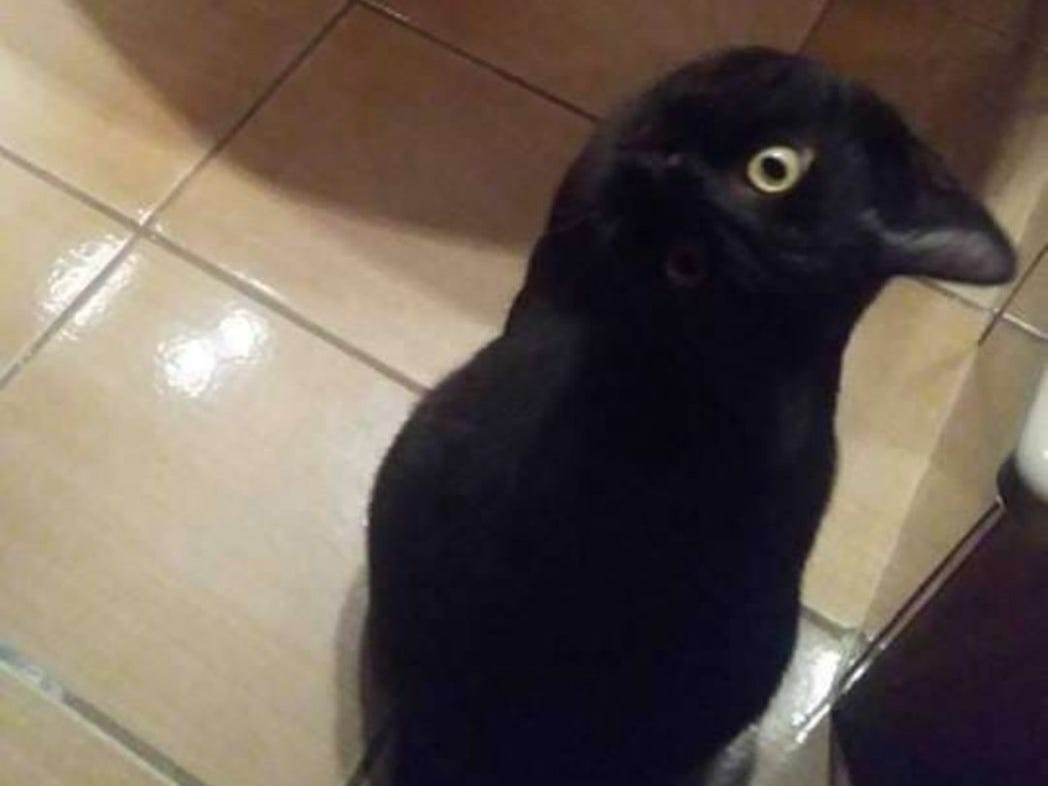
\includegraphics[width=0.5\textwidth]{Figs/litReview/catcrow.jpeg}
\caption{A cat that looks like a crow.}
\label{fig:catcrow}

\end{figure}

On closer inspection, humans can easily tell that \autoref{fig:catcrow} is not a picture of a crow. This could be due to high level knowledge such as the nature of the environment: ``indoor'', or noticing other images features such as the cat's other eye which is not well lit. The use of high level knowledge to improve classification of this image comes down to what does a human expect to see in an ``indoor'' image. Noticing that the environment and the assumed class of the animal in the image do not match, then allows the human to search for other discrepancies to expalin this non-alignment.

\ac{ANN} classifiers do not have the ability to apply this sort of high level knowledge and can only rely on the information held in the pixels . \acp{ANN} also do not look at high level features such as the ones I have described. In a \ac{ConvNet} the size of features the network is sensitive to are determined by the size of the kernels used in each layer (typically 3x3 - 7x7), in the first layer, these are very small image regions. The \ac{ConvNet} gains its expressive power by combining these features at greater and greater scale after each successive layer. However, this approach means that if a neuron in the early layers of the network is fooled into ``seeing'' a feature, this error is propogated upwards. This makes it easy to fool \acp{ANN} as they cannot take a top down approach to reason about the detected features. A top down approach relies on symbol grounding \cite{barsalou2008grounded}, which I will discuss later.



\subsection{Data Ineffciency}
As demonstrated by WaveNet's poor performance at representing Mandarin speech \cite{wavenet} when \acp{ANN} are not provided with enough data they often overfit and fail to distinguish between salient features and local noise in the training data. A large portion of the success of AlexNet \cite{krizhevsky2012imagenet} is due to the 1.2 million images that were used to train it. This was only possible due to the advancement of \ac{GPU} technology allowing for parallel computation of each convolution in the network. Attempting to train AlexNet on a \ac{CPU} would take a very long time.

Similarly, Vinyals et al. \cite{vinyals2015show} report that their image captioning system required millions of training instances to achieve their then state-of-the-art performance, even after pretraining on the 1.2 million images from ImageNet \cite{ImNet}.

Ha et al. \cite{ha2018world, ha2018recurrent} do show that pretraining an unsupervised world representation can allow for rapidly producing controllers capable of solving reinforcement learning tasks. However this is not generalisable to all problem spaces.

Obviously, \acp{ANN} are not comparable to adult humans when it comes to learning complex, high level tasks with little or no training. It is expected that an adult human could recognise a novel object and its name from a single training example, this is not to be expected from an \ac{ANN}.

Ha's approach of producing a compressed and feature rich representation of the world \cite{ha2018world, ha2018recurrent} may offer insight into how we can approach human like performance at one-shot-learning \cite{vinyals2016matching}. As demonstrated in the representation learning literature, pre-learning a representation which fulfils the criteria layed out in \cite{repRev} can greatly simplify many machine learning tasks.


\section{Getting off the Symbol Grounding Merry-Go-Round} 
In \cite{searle1980minds} Searle presents a thought experiment known as the Chinese Room Argument. In the thought experiment, he has the reader imagine a room in which an english speaker waits with a book of rules written in english explaining how to respond to any given set of Chinese characters. Outside of the room a native Chinese speaker passes notes into the room and waits for a note in return from the person inside the room. The person in the room uses the book of rules to craft a correct response without ever understanding the meaning of the symbols on the note. To the Chinese speaker, it seems that the person in the room understands Chinese, though they do not.

Searle posits that this shows that simply programming a computer to respond correctly to language is not enough to produce a machine which can understand and thus, the Turing Test \cite{turing2009computing} is inadequte to determine if a machine is truly intelligent.

The question, therefore, is ``How do we build a machine which can understand?''.

In order for a machine to understand the world, it must ground the symbols it manipulates within its program. In Searle's Chinese Room, the English speaker cannot ground the meaning of any of the Chinese symbols as they have no way of discerning the meaning of the symbols from their list of instructions. Whilst the instructions give the correct method for responding to each symbol these instructions are cyclic. Consider how you would discern the meaning of a word in a foreign language if you were given a dictionary of that language defining each word. You could look up a word and read the definition, however as the definition is also written in the foreign language you would need to look up the definitions of each word of the original definition, until eventually you wind up back where you started looking up the meaning of the original word \cite{cangelosi2000robotic}. This is the symbol grounding Merry-Go-Round: without being able to discern the meaning of at least one word in the dictionary, it is useless for enhancing your understanding of the language \cite{harnad1990symbol}.

In Serle's view, a purely computational system can never be truly intelligent without solving the symbol grounding problem. Whilst I agree with this, I believe it is not sufficient to just build a grounded system for it to be considered intelligent (as Searle would likely agree). As I will demonstrate in the experiments of this thesis, the \ac{MAE} is capable of learning a grounded representation of images and language, producing sensible output in one modaility when translating from the other. I would still not argue that this system is intelligent, though it has escaped the symbol grounding merry-go-round, it is still at its heart, a set of matrix multiplications (as detailed in \autoref{Chapter2}). To be considered intelligent, I would require the system to not only be grounded but to also exhibit directed action towards solving the task it has been set. That is, the system would need to demonstrate that it is aware of the problem it is solving, clearly this cannot be achieved through gradient descent and backpropagation, as it is the optimiser which adjusts the weights of the system, not the system itself.

\subsection{What is Symbol Grounding?}
Symbol grounding is the process of assigning meaning to a symbol. It is something babies and even animals are very good at. Despite not having access to a dictionary explaining the meaning of each word in terms of their internal symbolic representations, babies are able to learn to speak. Similarly, animals can learn the meaning of words, for example, sit, fetch, walkies...

How babies and animals do this will be explored shortly and I will explain how this can be applied to a robot to have it learn a grounded representation of its world.

In \cite{steels2008symbol}, Luc Steels explores the symbol grounding problem through the use of Semiotic Networks. \autoref{fig:semNet} shows a semiotic network, objects are connected to their symbols and the concepts which represent them.

\begin{figure}
\centering
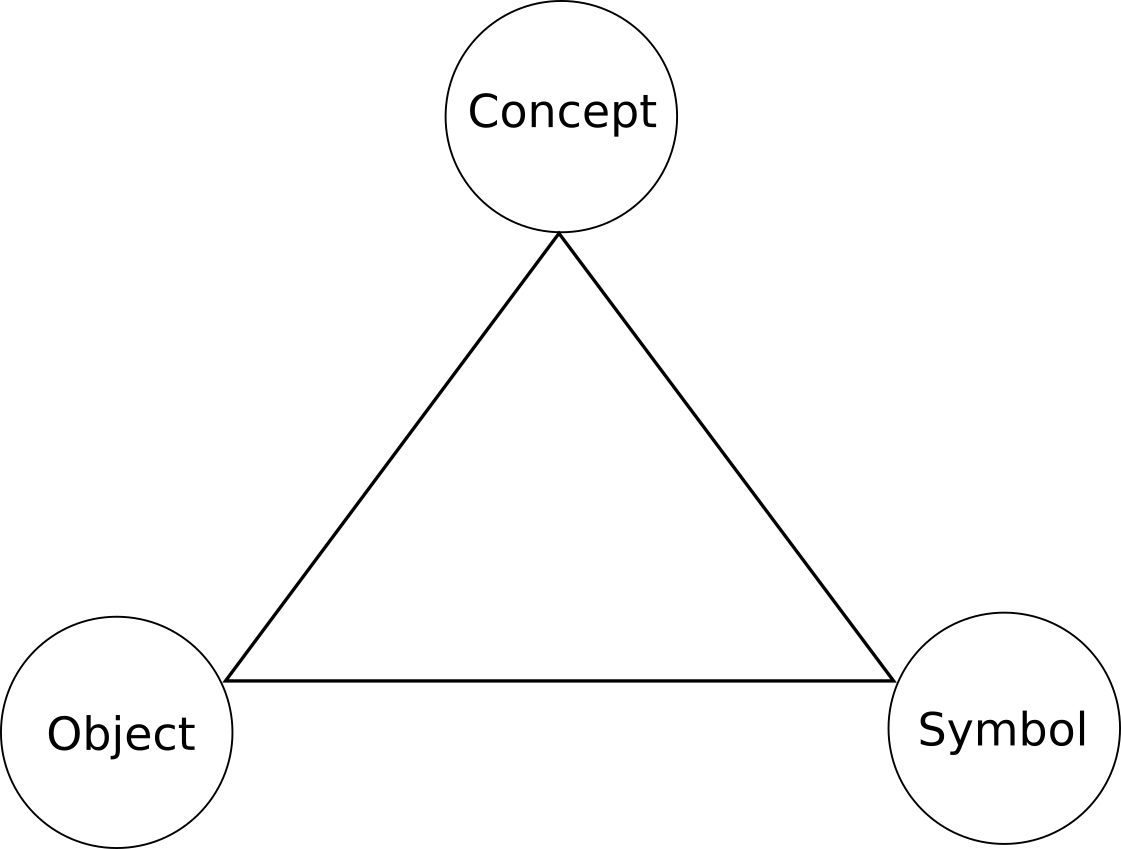
\includegraphics[width=0.5\textwidth]{Figs/litReview/semioticNet.png}
\caption{A Semiotic Network.}
\label{fig:semNet}

\end{figure} 

Semiotic Networks are useful for visualising the symbol grounding problem. They demonstrate what we are trying to achieve through symbol grounding; namely to develop methods to relate sensory percepts of the world and objects in it, to symbols via internal representations (concepts). Whilst this explanation implies some directionality to the network, there should not be. A system capable of grounding symbols should be able to move freely between symbols, concepts and objects. For example, given the words \textsc{Blue Ball} a person is capable or recognising the referrent object  \textit{Blue Ball} as well as the concepts ``Blue'' and ``Ball'' as well as preforming the reverse operation of nameing the object \textit{Blue Ball} with the words \textsc{blue ball}.

Now that I have explained what symbol grounding is, we can see how the following literature informs the experimental design process I undertook in order to test hypotheses 1 and 3 - \ac{MRL} can be used to learn the association between sounds and the visual symbols they represent. I.e. to solve the symbol grounding problem and \ac{MRL} can be used to learn language as it relates to the visual properties of objects. I.e. to solve the symbol grounding problem.


\subsection{How do Humans do it?}
Brains have many advantages over \acp{ANN} when it comes to the symbol grounding problem. The more prominent of these are, multimodality \cite{barsalou2008grounded}, sensory redundancy \cite{slater1999intermodal}, innate signal conditioning systems \cite{masland2012neuronal, fantz1963pattern, johnson2015two}, developmental learning (both pre \cite{webb2015mother, reid2017human} and post-natal \cite{johnson2015two}) and embodiment \cite{pfeifer2006body, smith2005development}.

Lawrence Barsalou \cite{barsalou2008grounded} takes the view that amodal symbol processing, that is ungrounded symbol processing is not how brains work. Instead, he suggests that cognition is performed through multimodal simulation of sensory percepts. He gives the example of sitting down onto a chair: as this experience occurs the brain captures states across the different sensory modalities and encodes these into a representation which can be stored in memory. When the representation of the chair is needed, the multimodal representation captured during the earlier experience is replayed as a simulation. Thus a person's representation of a chair is the sum of the representations of all of the experiences a person has had with chairs. 

Through this simulation process, the brain can compare whether a new experience belongs to a certain category by comparing its representation with the stored representation of the experiences of that categorey. The representation of expirences are likely stored, not like data in a computer but in the connections between neurons, I will refer to this as ensemble encoding \cite{nicolelis1995sensorimotor} and it is analogous to how the weights of neural networks encode features from the data they are trained on \cite{mordvintsev2015inceptionism}.


From Barsalou's work, we can see that in biological systems, symbol grounding is the process of linking percepts from different modalities (visual, sensorimotor, auditory, etc. as well as emotions and other internal bodily states), into a single representation. Therefore to test hypthesis 1 and 3, I will need to demonstrate that the \acp{MAE} are able to correctly translate from one modaility to the other and vice-versa.

\subsubsection{Embodiment}
\label{sec:embodi}
\begin{displayquote}
We are embodied; nothing more. - Arthur M. Glenberg
\end{displayquote}
Embodiment - that is, having a body - is a vital part of human cognition. It is embodiment that allows humans to ground symbols by associating symbols in perception action and emotion, giving them meaning \cite{glenberg2015few}.

By learning to associate different sensory percepts with one and other as well as with world states, humans learn a grounded world model \cite{barsalou2008grounded}. The body mediates the learning of this representation, as the sensors from which the representation arises are (part of) the body. 

Glenberg \cite{glenberg2015few} views the comprehension of symbols as a simulation process, in line with Barsalou's views on this matter \cite{barsalou2008grounded}. By simulating the percepts associated with a symbol via the mirror neuron system, the brain is able to understand the meaning of the symbol.


In \cite{pfeifer2006body}, Pfeifer et al. go as far as to say that intelligence requires embodiment. Mathematical reasoning is often seen as an intelligent behaviour and as computers, which are not embodied, are capable of performing mathematical operations, this idea is contradicted. However, in humans, mathematics is performed in an embodied and grounded manner.  

There have been numerous studies of both children and robots, showing that use and observation of gestures significantly aids learning of abstract numerical concepts, so much so that prohibiting gesture detriments comprehension \cite{Goldin-MeadowSusan2015Fata, de2014making, rucinski2012robotic}. This highlights how the body can be used to enable grounded cognition.

Whilst I agree that embodiment can facilitate symbol grounding and therefore intelligence I do not agree that it is required for intelligence. It is easy to imagine an artificial system which is capable of intelligent action without a physical body. For example, a program designed to trade on the stock market could be considered intelligent so long as it is aware of what it is doing and why it is doing it. Whilst this is not how such systems are designed, as it is much simpler to design a program to mathematically optimise a cost function than one which is aware of the task it has been set, it is possible that in future a different design paradigm could be followed.

\subsection{Multimodality}
One key aspect of emboidment is that it makes all experiences multimodal. Even if only a single sensor is being actively used in a given activity, all of the bodies sensors and its internal state are involved in the experience. 
In the case of learning to count, the use of gestures, such as counting on fingers, introduces the sensory-motor system as a source of information from which a grounded symbol for each number can arise. For example the abstract symbol ``1'' is associated with the auditory percept of the word ``one'' as well as the gesture of raising a single finger, creating a rich, multimodal encoding of the symbol in the brain.

The use of multimodal information for distinguishing between symbols (e.g. numbers) clearly enhances learning by providing a richer representation of the symbol. This relates directly to hypothesis 2 - \ac{MRL} enhances classification accuracy of sounds and visual symbols, where I will test whether multimodality improves calssification accuracy. As demonstrated in both the human and robotics related literature, multimodality can improve classification accuracy.

Multimodality also improves learning by providing an attention mechanism \cite{bahrick2000intersensory}. The synchrony of signals from different sensors guide infant attention to salient information. This idea is supported by studies examining how infants learn to speak.  Smith et al. \cite{smith2008infants} demonstrate that infants preferentailly looked at target images over distractor images guided by an auditory cue (the name of the target image). Several other studies have demonstrated a similar result \cite{walker2010preverbal, fischer2011multi, scott20122, slater1999intermodal}.

The work of Smith et al. clearly demonstrates that multimodality plays a key role in how humans learn language, therefore it should play a key role in how robots learn language too.

In \cite{lupyan2007reuniting}, Lupyan explores the effect of aural, linguistic labelling on the response time of adults on a symbol search task. Two experiments were performed, in the first participants were shown displays containing images of  unfamiliar symbols (\rotatebox[origin=c]{90}{2} and \rotatebox[origin=c]{90}{5}) and instructed to locate a target symbol. In the second experiment participants were shown displays of familiar or unfamiliar symbols (2, 5, \rotatebox[origin=c]{90}{2} and \rotatebox[origin=c]{90}{5})) and told to either find or ignore a target symbol. For example, a display containing many 5s and a single two would be preceded by the aural instruction ``find the 2'' or ``ignore the 5''.

Participants in experiment 1 who reported labelling the unfamilar symbols had a significantly faster response time than those who did not. Similarly in experiment 2 a significant effect was seen on the familiarity of symbols, with both 2 and 5 being easier to locate than both \rotatebox[origin=c]{90}{2} and \rotatebox[origin=c]{90}{5}.

\begin{displayquote}
...a learned category label becomes
strongly associated with features that are most diagnostic (or
typical) of the named category, using the label can in effect
make an object a “better” object by augmenting its idiosyncratic perceptual features with features typical to the named
category. - Gary Lupyan
\end{displayquote}

The above quote from Lupyan helps explain why familiar, labelled, symbols are easier to locate than those which are unfamilar and why labelling unfamilar symbols leads to a similar improvement in response time. By labelling a symbol (in this case a visual pattern on a screen), the representation of the symbol is altered into a more recognisable form. 
I will demonstrate a similar effect in \autoref{Chapter4} where the addition of an aural labelling leads to the generation of images of more prototypical digits than relying on the visual stimuli alone. The effect of adding a secondary modality, i.e. the mental labelling applied in experiment 1 of \cite{lupyan2007reuniting}, is to bring the representation of the visual symbol closer to a familiar, easily recognisable representation.

\subsection{Development}
Another advantage that humans have over \acp{ANN} is that their learning occurs in a developmental fashion. Whilst \acp{ANN} are typically expected to go from random initialisation to super-human performance without any incremental stages between, humans are allowed to gradually develop new skills over the course of a lifetime, bootstrapping new abilities on top of previous ones. We do not expect babies to be able to count, let alone do advanced mathematics - why then do we expect this of \acp{ANN}.

Developmental learning occurs, not just after birth but also pre-natally. In \cite{webb2015mother}, Webb et al. explore how the mother's voice and heartbeat contribute to the development of the infant brain's auditory processing abilities. By playing recordings of the mothers' voices and heartbeats to preterm babies, an increase in the size of the auditory cortex was seen versus preterm infants who heard only unfiltered, background hosptial noise.


In \cite{fantz1963pattern}, Fantz showed in 1963, that newborn infants have acute pattern sensitve vision. With the development of new technologies, Reid et al. \cite{reid2017human} were able to determine that human fetuses preferentially look at face-like stimuli inutero. Suggesting that development of the visual systems begin before birth.

These studies demonstrate how human infants do not start off with a random configuration of the brain when they are born and thus even they have an advantage over \acp{ANN} due to developmental processes.

Infants are then given years of training to learn to be the adaptable, general intelligences that they are. Parents aid this through the use of specific infant directed behaviours such as `Motherese' \cite{fernald1987acoustic} and looming actions \cite{lohan2012contingency, lohan2012tutor}. Followed by teachers, peers and the general structure of society shaping their learning.

In order to demonstrate that a developmental approach to learning can aid in machine learning, I take an incremental approach to the solving the symbol grounding problem in \autoref{Chapter5}, testing Hypothesis 4 - \ac{MRL} can be improved through transfer learning. 

\paragraph{Biological Filters}
As a consequence of embodiement, humans have inherent signal conditioning systems \cite{pezzulo2013computational}, these help guide the learning process.

In \cite{johnson2015two}, Johnson et al. comment on the well established `\ac{TPT} of face processing' in humans.  During the `Conspec' stage of the \ac{TPT} the superior colliculus interacts with both visual and motor systems driving visual attention towards conspecific stimuli. The `Conlern' stage of the \ac{TPT} is guided by the `Conspec' stage due to a larger proportion of conspecific visual data  (e.g. the human face) being provided to the visual cortex as more attention is given to these stimuli by the superior colliculus. 
The superior colliculus guides learning in the visual cortex by controlling attention.

In \cite{bambach2017egocentric}, Bambach highlights the importance of data quality when training visual recognition systems, thus the superior colliculus may help to improve the learning of the visual cortex by providing focused, high-quality training examples. 

Testing the \ac{TPT} is much simpler in artificial models thus, approaches like that of \cite{bambach2017egocentric} should be adapted to enhance our understanding of human development and learning.

As well as the structure of the human brain which has been optimised by evolution to facilitate rapid learning, the physical embodiment of humans guides and improves human learning. Possibly the best example of this is the human eye, specifically the retina.

The highly organised nature of the retina predisposes the types of visual data presented to the visual cortex to have certain characteristics through signal conditioning, as well as shape and movement specific sensitivity \cite{masland2012neuronal}.

Signal conditioning in the retina enhances object boundary detection by reducing the brightness of the brightest areas and their immediate surroundings, giving objects an outline. Other effects in the retina are sensitive to movement and help segment the background from moving objects in the foreground \cite{olveczky2003segregation}.

Similarly, the shape of the human ear and the physical structure of the inner ear filters and shapes the sounds we hear which facilitates learning and detection of relevant sounds whilst reducing the perception of background noise \cite{oxenham2018we}.

Differentiating between the effects of developmental processes and the innate signal conditioning provided by the human body is difficult, though it can be seen that these are two separate effects. This is demonstrated, for example, by the increase in auditory cortex volume in preterm babies in \cite{webb2015mother}. Demonstrating the difference between these effects in \acp{ANN} is more difficult. As \acp{ANN} lack an embodiment, they do not have innate signal conditioning systems, either feature engineering needs to be done to simulate this, or pretraining can be performed to create a set of \ac{ANN} weights which extract the relevant features. The issue here is that pretraining can also be seen as part of the developmental process.

Whilst the human body has had millenia of evolution to shape the signal processing systems and the initial neural connections of the brain, neural networks do not have this luxury. Thus, to keep things simple, I will refer to pretraining of \acp{ANN} as if it were wholely an anology of developmental processes. However, I think it is worth noting that the pretraining step can be viewed as analogous to the evolutionary processes which have shaped the innate signal conditioning which occurs in human sense organs.

\subsection{How do Machines do it?}
Symbol grounding has been tackled in many different ways by different groups within the scientific community. Notably this is because different groups holding differing ideas about what constitutes symbol grounding and how grounded symbols should be used by Artificial Intelligence. Both Barsalou \cite{barsalou2008grounded} and Cangelosi \cite{cangelosi2000robotic} take the stance that amodal symbolic manipulation systems are not good models of how brains operate. This is contrary to the views of the \ac{NLP} community on cognition and symbol grounding \cite{lemonlearning, yu2017learning}.

Whilst Cangelosi et al. note that categorical representations are sensory rather than symbolic as they preserve some of the ``shape'' of the sensory projections, they are not used in this way within the \ac{NLP} systems of \cite{lemonlearning} and \cite{yu2017learning}. I would argue that by converting from a probability distribution across possible categories to amodal symbols, all grounding is lost in these \ac{NLP} systems.

Coradeschi et al. \cite{coradeschi2000anchoring, coradeschi2003introduction} would refer to this style of ``grounding'' as Anchoring. Anochring is the process of linking a sensory percept to a symbol. However as there is no way for the system to link back from the symbol to the sensory percept, it clearly is not grounded. This is demonstrated in \autoref{fig:ank}, where it can be seen that not only does this network lack a ``Concept'' node (the node repsonsible for allowing the system to understand the meaning of a symbol and percept) but also that there is a directional constraint which should not be present in a grounded semiotic network. 

\begin{figure}
\centering
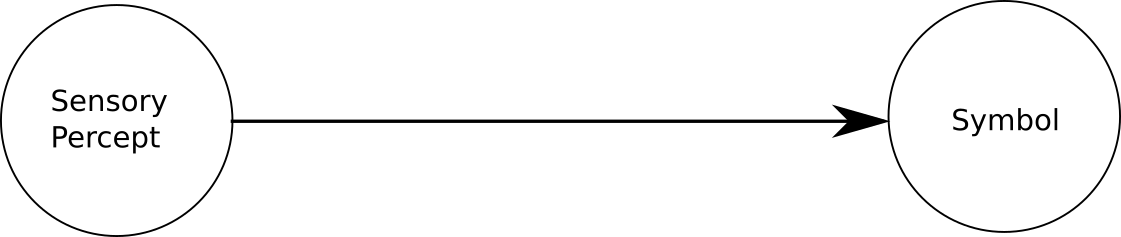
\includegraphics[width=0.5\textwidth]{Figs/litReview/anchoring.png}
\caption{A depiction of Anchoring relative to a Semiotic Network.}
\label{fig:ank}

\end{figure}


In \cite{coradeschi2013short}, Coradeschi et al. present two forms of symbol grounding, physical and social. Physical symbol grounding is the grounding of symbols to real world objects by a physical agent in the real world \cite{vogt2002physical}; whereas social grounding is the collective negotiation of the meanings of shared symbols in groups of agents \cite{cangelosi2006grounding} (e.g. how natural language evolves over time).

An important note from Coradeschi's review \cite{coradeschi2013short} is that ``symbol grounding is a bidirectional process'', again, this is in direct conflict to the view shown in \cite{lemonlearning, yu2017learning}. Later in this work, I will explicitly use the term bidirectional grounding to highlight the capabilities of \ac{MRL} as applied to physical symbol grounding.

Further to this, Coradeschi et al. discuss methods which utilise both visual and auditory data which were demonstrated to have better performance at object categorisation than systems using only a single modality \cite{coradeschi2013short}. These multimodal systems perform physical symbol grounding as an inherent property of their oporation. By learning a joint representation of the two modalities an internal ``Symbolic Language'' is created. These systems are shown to have capabilties beyond simply categorising objects or words. They can be used to facilitate meaningful conversation between humans and the robots which use them \cite{nakamura2009grounding, nakamura2011grounding}. Cangelosi et al. also present a system capable of grounding symbols with the sensory percepts to which they relate \cite{cangelosi2000robotic}. Through the use of \acp{ANN}, a joint representation of symbols and visual stimuli is learnt.

Multimodal approaches to symbol grounding, in my opinion, are both natural and more flexible than systems which attempt to use amodal symbols derived from a single modality.

\begin{displayquote}
``Symbol systems alone are not viable models of the mind... connections between its symbols and what they stand for must be direct and intrinsic to the system.'' - Cangelosi et al.
\end{displayquote}

The above quote highlights why learning a multimodal representation of symbols and sensory percepts solves the symbol grounding problem. In learning a joint representation, a symbol and sensory percept are grounded to a single concept within the network, i.e. their representation.

\autoref{fig:percNet} shows a modified semiotic network depicting Cangelosi et al.'s approach to symbol grounding by learning a joint representation \cite{cangelosi2000robotic}. By comparing \autoref{fig:semNet} and \autoref{fig:percNet} it can be seen that there is a missing link between the Sensory Percept and the Symbol. Cangelosi et. al recreate this link by regenerating both the symbol and the sensory percept at the output of the \acp{ANN} from the joint representation. This autoencoding approach is how I address the symbol grounding problem later in this thesis.

\begin{figure}
\centering
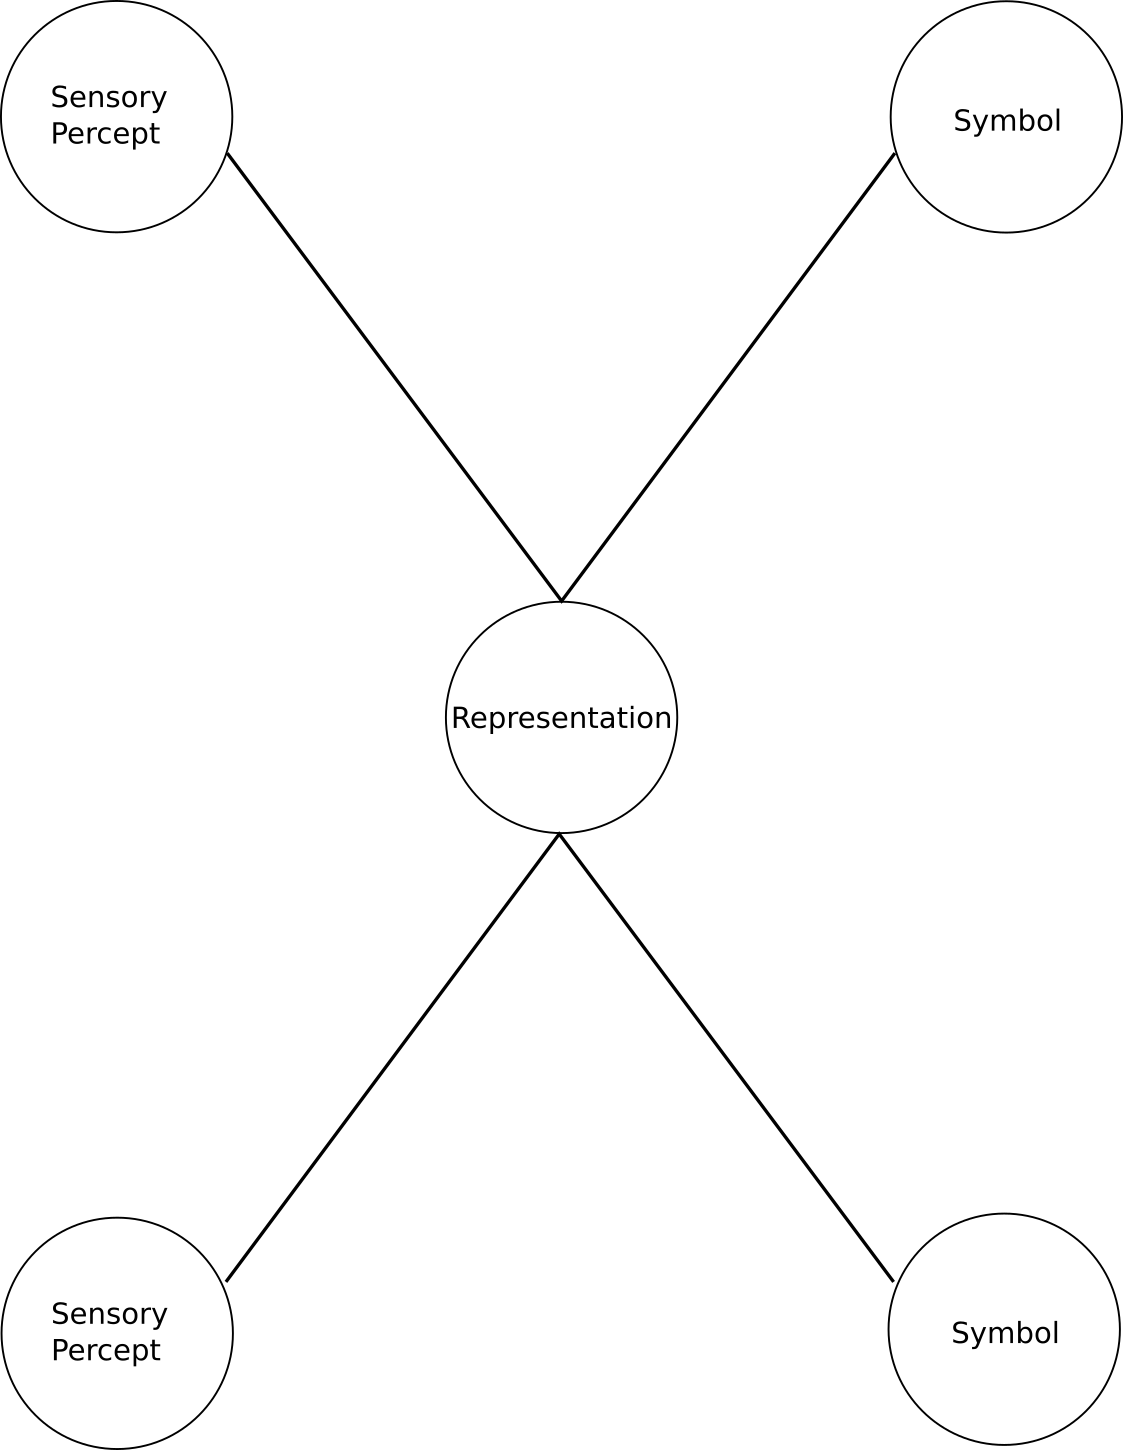
\includegraphics[width=0.5\textwidth]{Figs/litReview/semioticNetPercept.png}
\caption{A Semiotic Network modified to demonstrate Cangelosi et al.'s approach to symbol grounding.}
\label{fig:percNet}

\end{figure}


As well as physical symbol grounding, Cangelosi et al. have worked on social symbol grounding \cite{cangelosi2001adaptive, cangelosi2002symbol, cangelosi1998emergence, horst2019object, cangelosi2018speech, cangelosi2008italk, broz2014italk}.

In \cite{cangelosi1998emergence} Cangelosi et al. have a population of \ac{ANN} based agents which learn to communicate about whether mushrooms are either safe to eat or poisonous. In order to reproduce, the \acp{ANN} must avoid eating poisonous mushrooms. Thus, \acp{ANN} which can comunicate which mushrooms are poisonous and which are safe to eat have an evolutionary advantage. 

Through this evolutionary process, the \acp{ANN} learn to agree on a set of symbols which indicate which mushrooms are safe to eat. This is social symbol grounding in practice. 

This method for developing a symbolic language to maximise a reward function, is analogous to the process which occurs between the two networks in Vinyal's image captioning system \cite{vinyals2015show}.  The two networks, image encoder and language model respectively, must learn a shared symbolic language which will allow the combined network to generate accurate image captions.


\subsubsection{My Approach to Symbol Grounding}

In my opinion, multimodality is fundamental to symbol grounding and is a key aspect of embodiment. The work in this thesis focuses on the grounding of visual and linguistic percepts and does not explore how actions, emotions or other more complex phenomina should be modeled in a grounded manner. I use datasets of paired visual and linguistic percepts to train \acp{MAE}. The future work section details how my approach can be extended for operation in the real world with the use of a robot body. This approach builds off of the work of Ngiam et al. \cite{ngiam2011multimodal} and Silberer et al. \cite{silberer2014learning} on \acp{MAE}, in particular.

\subsubsection{Why use MAEs?}
In \cite{ngiam2011multimodal}, Ngiam et al. train a \ac{MAE} using video and pre-processed audio data to classify speech data. They demonstrate that the addition of the visual data improves recognition under noisy conditions, highlighting the technical advantages of \acp{MAE}. Further to this they demonstrate that the McGurk effect \cite{mcgurk1976hearing} occurs in the \ac{MAE}, highlighting that it is a good analogy for the human audio and visual cortices and how they interact.
Somewhat surprisingly, Ngiam et al. only find an improvement to classification under noisy conditions when multimodal data is used to classify phonemes, compared to a unimodal baseline. In \cite{barsalou2008grounded}, Barsalou explains how multimodal percepts of a single phenomenom should have two advantages over unimodal percepts. 1) They provide information redundancy, thus in noisy conditions, any information lost from one modality due to the noise can be recovered from the other modality(s), and 2) each modality should contain its own unique information which can be used to aid  classification of the phenomenom.
From these two factors, I would expect that multimodality would enhance classification under all conditions, not just noisy ones. I, therefore, would suggest that there may be an issue related to the capacity of the \ac{MAE} designed by Ngiam et al. which could have benefitted from having additional layers or neurons added to it. This would allow for a more complete representation of the multimodal percepts with which it is trained.

In \cite{silberer2014learning}, Silberer et al. demonstrate the ability of \acp{MAE} to reconstruct missing data when only one modality is present. A similar effect is seen in the human brain where sensory redundancy is utilised to repair and reconstruct data from noisy or missing percepts \cite{samuel1997lexical}.  In my opinion, a key draw back of Silberer et al.'s approach is their use of image tags in place of natural language. Whilst image tags are useful for image retrieval tasks they are less useful in a robotics setting. Humans communicate using natural language descriptions of the objects and scenes they see, not with image tags. As I aim to develop a system which can be used to facilitate \acl{HRI}, I will be working directedly with natural language.  

\subsubsection{Transfer Learning and Pretraining}

Barsalou \cite{barsalou2008grounded} does not believe that the brain is started from a competely random configuration:
\begin{displayquote}
``...there are no a priori reasons why simulation cannot have a strong genetic basis. Genetic contributions almost certainly shape the modal systems and memory systems which capture and implement simulations'' - Lawrence Barsalou.
\end{displayquote}

This is important as it sheds light on why \acp{ANN} require much more data to perform tasks which would take a human baby very little time to master. 

The cognitive development of infants can be simulated through pretraining. In \cite{lee2008sparse} pretraining of \acp{ANN} is demonstrated to give rise to Gabor like filters similar to those seen in the human visual cortex. These pretrained filters make high level tasks easier. For example, in \cite{vinyals2015show}, Vinyals et al. demonstrated that by pretraining an image feature extraction network on an image classification task and a language model on a word prediction task, the combined network was able to produce correct captions for images with a  relatively small amount of direct training. 

The effect of transfer learning from one task to another is that it moves the weights of the network away from their random starting values towards a configuration which is closer to the optimal values. This allows the \ac{ANN} to start in a configuration which is closer to the starting configuration of an infant brain which is shaped by genetics and evolutionary processes \cite{barsalou2008grounded}.


\section{Research Plan}
The rest of this thesis is organised into 3 experimental chapters followed by a conclusion and future work chapter.
Each of the experimental chapters address one or more of the hypothesis of this thesis.

To reiterate, the hypothesis are:

\begin{enumerate}

	\item \ac{MRL} can be used to learn the association between sounds and the visual symbols they represent. I.e. to solve the symbol grounding problem.
	\item \ac{MRL} enhances classification accuracy of sounds and visual symbols.
	\item \ac{MRL} can be used to learn language as it relates to the visual properties of objects. I.e. to solve the symbol grounding problem.
	\item \ac{MRL} can be improved through transfer learning.
	\item The multimodal representation learnt by the \acp{MAE} exhibits the desirable properties of a representation as layed out by Bengio et al. in \cite{repRev}.		
	\item It is possible to use \ac{MRL} with real data.
	
\end{enumerate}

Chapter 4 focuses on hypotheses 1 and 2, making use of MNIST Handwritten Digits and UCU Arabic Spoken Digits datasets to do this. Chapter 4 is concerned with demonstrating the feasability of the technical approach taken as well as validating design choices made based on the findings of the literature review. 

Chapters \ref{Chapter5} and \ref{Chapter6} primarily focus on exploring how linguistic and visual symbolgrounding can be achieved. Chapter \ref{Chapter5} explores the effects of transfer learning (hypothesis 4), relating the results to the findings of the developmental literature and evaluates the quality of the learnt representation, comparing to the criteria layed out in \cite{repRev}. In \autoref{Chapter6}, I demonstrate how \ac{MRL} can be used to achieve the bidirectional grounding of real data (hypothesis 6). 
